\documentclass{article}
\title{CS 279 Assignment 2: Conduct an Experiment\\Part 2: Laboratory study}
\author{Miriam Cha and Melih Elibol}
\date{September 23, 2014}

\usepackage{amsmath}
\usepackage{bbm}
\usepackage{fullpage}
\usepackage{graphicx}
\usepackage{listings}
\usepackage[usenames,dvipsnames]{color}

\usepackage{amsmath,graphicx,amssymb,amsfonts,bbm,subfigure}
\usepackage{array,colortbl,xcolor}

\usepackage{tikz}
\usetikzlibrary{shapes,arrows}
\usepackage{caption}
\usepackage{multirow}
\usepackage{color, colortbl}
\definecolor{lightgray}{gray}{0.9}

\begin{document}
\maketitle

\section*{Figure and Table} 

\begin{figure}[tbh]
    \centering
    \subfigure[Task time]
    {
    %left, bottom, right, top%
    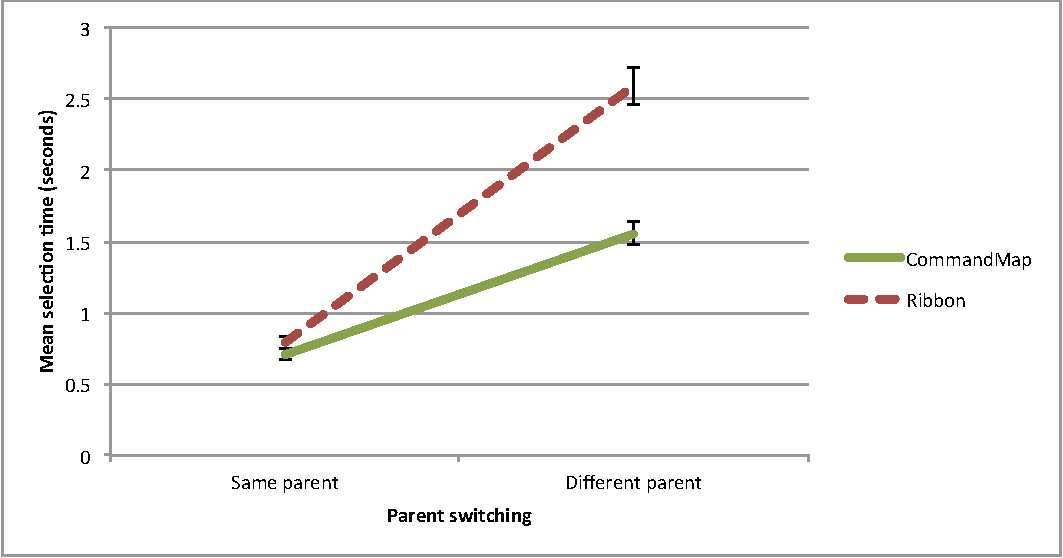
\includegraphics[trim = 0mm 0mm 0mm 0mm, clip,width=80mm]{figure5a.pdf}
    }
    \subfigure[Errors]
    {
    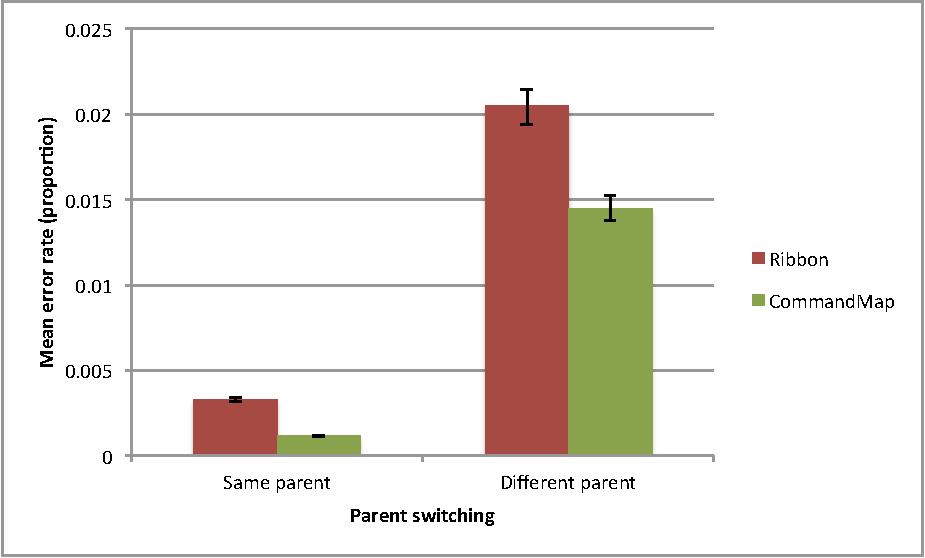
\includegraphics[trim = 0mm 0mm 0mm 0mm, clip,width=70mm]{figure5b.pdf}
    }
    \caption{Restults for Study 2, with (a) shown as a line chart and (b) shown as a bar chart for consistency with Figure 5 in the original paper. Error bars show standard error.}
    \label{fig:result1}
\end{figure}

 \begin{table}[tbh]
  \centering
\begin{tabular}{c|c|c|c|c}
  &  \textbf{Ribbon}  &  \textbf{CM} &  \textbf{$\chi^2$} & \textbf{Sig}          \\\hline
 \textbf{Mental demand}&   2.7 (1.2)  & 2.2 (1.2)  & 16.7  & $<0.06$   \\ \hline
 \rowcolor{lightgray}
\textbf{Physical demand}  &    1.9 (1.2) &   1.5 (0.5) & 4.1  & $<0.2$  \\\hline       
\textbf{Temporal demand}  &    3.2 (1.1) &   3.3 (1.0) & 22.4  & $<0.04$  \\\hline      
 \rowcolor{lightgray}
\textbf{Hard work}  &    2.8 (1.1) &   2.7 (1.1) & 20.0  & $<0.02$   \\\hline   
\textbf{Frustration}  &    1.9 (0.7) &   1.5 (0.7) & 7.3  & $<0.2$ \\ \hline \hline
\end{tabular}
\caption{Mean (st. dev.) NASA-TLX values (1=low, 5=high)}
\label{fig:trial_log}
\end{table}


%Upon completion of each interface, participants complete NASA-TLX worksheet to assess workloads. Table~\ref{fig:nasa_log} shows notional log entries for NASA-TLX. At the end of an experiment, participant chooses an interface for preference. Entry logs similar to Table~\ref{fig:nasa_log} and Table~\ref{fig:pref_log} are gathered to find support for $H_3$.   
%\begin{table}[tbh]
%  \centering
%\begin{tabular}{|l|c|c|c|c|c|c|c|c|}
%  \hline
%  ID &  Interface  & Mental 	&  Physical 	 &Temporal  	& Hard  & Frustration      \\      
%       &                  & Demand	& Demand 	& Demand 	& Work		     &			\\\hline
%$3234$ &   Ribbon  & $3$  & 2  & $2$ & 4  &2  \\ \hline
%$3234$  &    CM &   $2$ & 1  & $2$ & 2 &1  \\\hline       
%\end{tabular}
%\caption{Example of log entries for NASA-TLX}
%\label{fig:nasa_log}
%\end{table}
%
%\begin{table}[tbh]
%  \centering
%\begin{tabular}{|l|c|c|}
%  \hline
%    ID               & preference                \\\hline
% $3234$ &   CM      \\ \hline
%\end{tabular}
%\caption{Example of a  preference log entry per a participant}
%\label{fig:pref_log}
%\end{table}
%%%%%%%%%%%%%%%%%%%%%%%%%%%%%%%%%%%%%%%%%%%%
%
%
% %%%%%%%%%%%%%%%%%%%%%%%%%%%%%%%%%%%%%%%%%%
%\section*{Design Characterization}  
%\begin{itemize}
%   \item \textbf{\textit{Independent variables:}} \\
%   Interface 
%    \item \textbf{\textit{Dependent variables:}}\\
%    Selection time, error rate, NASA-TLX measures (mental demand, physical demand, temporal demand, hard work, frustration), and interface preference 
%    \item \textbf{\textit{Control variables:}} \\
%   User's familiarity in MS Word 2007, resolution, computer specs, and screen size
%   \item \textbf{\textit{Random variables:}} \\
%   Weather, temperature in the room, vision power of a participant, reaction rate of a participant, noise level, and usual versions of MS Word that a participant uses
%   \item \textbf{\textit{Design modification:}} \\
%   \textit{- Design modifications from what's described in the paper:}
%   Number and gender partitions of participants, computer specifications, screen size, and `correct' sound component in addition to `incorrect' sound.
%   \\
%   \textit{- Design choices that weren't clear in the paper that we had to figure out on your own:}
%   Methods of pointing (mouse, trackball, touchpad, joystick?), mouse acceleration, display of time, presentation methods of an instruction (``as quickly and accurately as possible"), audible deep sound, definition of error rate (CM inherently has a smaller number of total clicks if we include `tab clicks' into `total number of clicks.' Therefore, for Ribbon, we only count `command target clicks' into `total number of clicks'.) 
%   \end{itemize}
%
%\section*{Internal and External Validities}  
%\begin{itemize}
%   \item \textbf{\textit{Threat to internal validity; Can we mitigate them?; How?}} \\
%   If we were to perform experiments for Study 2 at anytime throughout a week, external environmental factors could threat internal validity. In order to mitigate potential threat to internal validity, we plan to perform experiments at the same time period throughout the week. Additionally, we will keep the same location, lighting, computer, mouse, keyboard, task, and presentation method of an instruction. 
%   \item \textbf{\textit{Threat to external validity; Can we mitigate them?; How?}} \\
%   Simply performing the experimental task of clicking command targets may not generalize to the world outside the lab that tends to include performing other additional tasks (e.g., email, doc edits, web browsing); For the purpose of replicating Study 2, this concern cannot be mitigated. It would be ideal if we can assess the similarity of the behaviors between the lab and the field but it is beyond the scope of Study 2.  However, we plan to conduct an experiment in a realistic environmental setting (e.g., MD office). In order to mitigate potential external validity on gender imbalance (in the original experiment, the proportion of male to female was 8 to 1), we plan to recruit male and female participants who are knowledge to MS Word with nearly equal numbers. 
%   \end{itemize} 
   

\end{document}
